\section{Vectors}
\paragraph{Vector notations}\ 

\begin{tabularx}{\textwidth}{l | X}
    Notation & Specs\\
    \hline\hline
    Magnitude-Angle notation & \tabeq{
        \vec{v} =\begin{cases}
            m \mbox{ - Magnitude}\\
            \sigma \mbox{ - Angle}
        \end{cases}
        \equiv \langle m, \sigma\rangle}\\
    \hline
    Component notation & \tabeq{
        \vec{v} = v_x \hat{i} + v_y \hat{j}\equiv \begin{bmatrix}   
            v_x\\ v_y
        \end{bmatrix}}\\
    \hline
\end{tabularx}
\paragraph{Vector operations}\ 

\begin{tabularx}{\textwidth}{l | X}
    Name & Equation \\
    \hline\hline
    Changing vector notation & \tabeq{
        \begin{cases}
            m = \sqrt{v_x^2 +v_y^2}\\
            \sigma = \tan\frac{v_y}{v_x}
        \end{cases}
        \iff
        \begin{cases}
            v_x = m \cos \sigma\\
            v_y = m \sin \sigma
        \end{cases}}\\
    \hline
    Unit vector & \tabeq{
        \hat{v} = \begin{cases}
            |v| = 1 \mbox{ - Magnitude-Angle notation}\\
            \frac{1}{|v|} \vec{v} \mbox{ - Component notation}
        \end{cases}}\\
    \hline
    Vector negation & \tabeq{
        -\vec{v} = \begin{cases}
            \langle m, \sigma + \pi\rangle \mbox{ -Mag/Angl}\\
            (-v_x, -v_y) \mbox{ -Comp.}
        \end{cases}}\\
    \hline
    Vector sum & \tabeq{
        \vec{a} + \vec{b} = (a_x + b_x, a_y + b_y)}\\
    \hline
    Scalar multiplication & \tabeq{
        a\vec{v} = \begin{cases}
            \langle|am|, \texttt{if } a\ge0:\sigma\texttt{ otherwise }\sigma+\pi\rangle\mbox{ -Mag/Angl}\\
            (av_x, av_y)\mbox{ -Comp.}
        \end{cases}}\\
    \hline
    Dot product & \tabeq{
        \vec{a}\cdot\vec{b} = \begin{cases}
            |a||b|\cos(\phi)\mbox{ -Mag/Angl}\\
            a_xb_x+a_yb_y\mbox{ -Comp.}
        \end{cases}}\\
    \hline
    Angle between two vectors & \tabeq{
        \cos(\phi) = \frac{\vec{a}\cdot\vec{b}}{|a||b|}}\\
    \hline
    Cross product & \tabeq{
        \vec{a}\times\vec{b} = \begin{cases}
            \langle |a||b|\sin(\phi), \sigma\mbox{ ortho. to inputs}\rangle\mbox{ -Mag/Angl}\\
            \begin{vmatrix}
                \hat{i}&\hat{j}&\hat{k}\\
                a_x&a_y&a_z\\
                b_x&b_y&b_z
            \end{vmatrix}=\begin{aligned}[c]
                (a_yb_z-a_zb_y)\hat{i} - (a_xb_z-a_zb_x)\hat{j}+\\(a_xb_y-a_yb_x)\hat{k}
            \end{aligned}
        \end{cases}}\\
    \hline
\end{tabularx}

\begin{wrapfigure}[8]{r}{0.3\textwidth}
    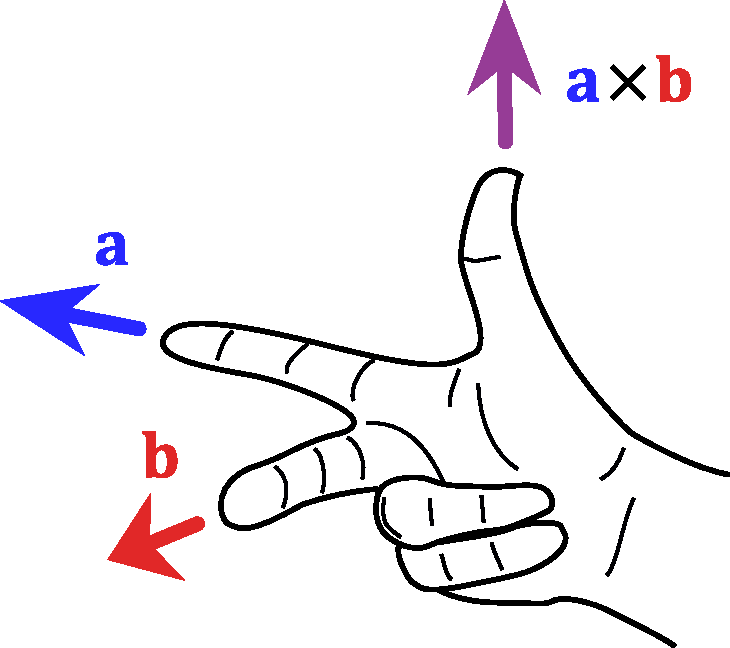
\includegraphics[width=0.3\textwidth]{chapters/vectors/images/right_hand_rule.pdf}
\end{wrapfigure}
\subparagraph{Right-hand rule} The right-hand rule is a simple way to imagine the direction of the vector resulting off a cross product, indeed it is not easy to find it through the Magnitude-Angle notation, nor it is so through Component notation (even though by crunching the numbers it is possible to do so). If done well it is easy to visualize how impossible it is to process the same result by switching the arguments: spoiler it would be of the opposite direction.